\section{Model of the controlled system}
\label{system_design}

The system was previously introduced in detail through the block diagram shown in \figref{fig:gensetmodeling}. It should be considered however, that it is complicated and unnecessary to handle a system in such a detailed form, therefore a more compact system description is required. In order to restructure the model and get a more convenient form, the inner processes can be represented with their transfer functions, thus combined in a subsystem such as in \figref{fig:blok_simplified}

%\begin{figure}[H]
%\centering
%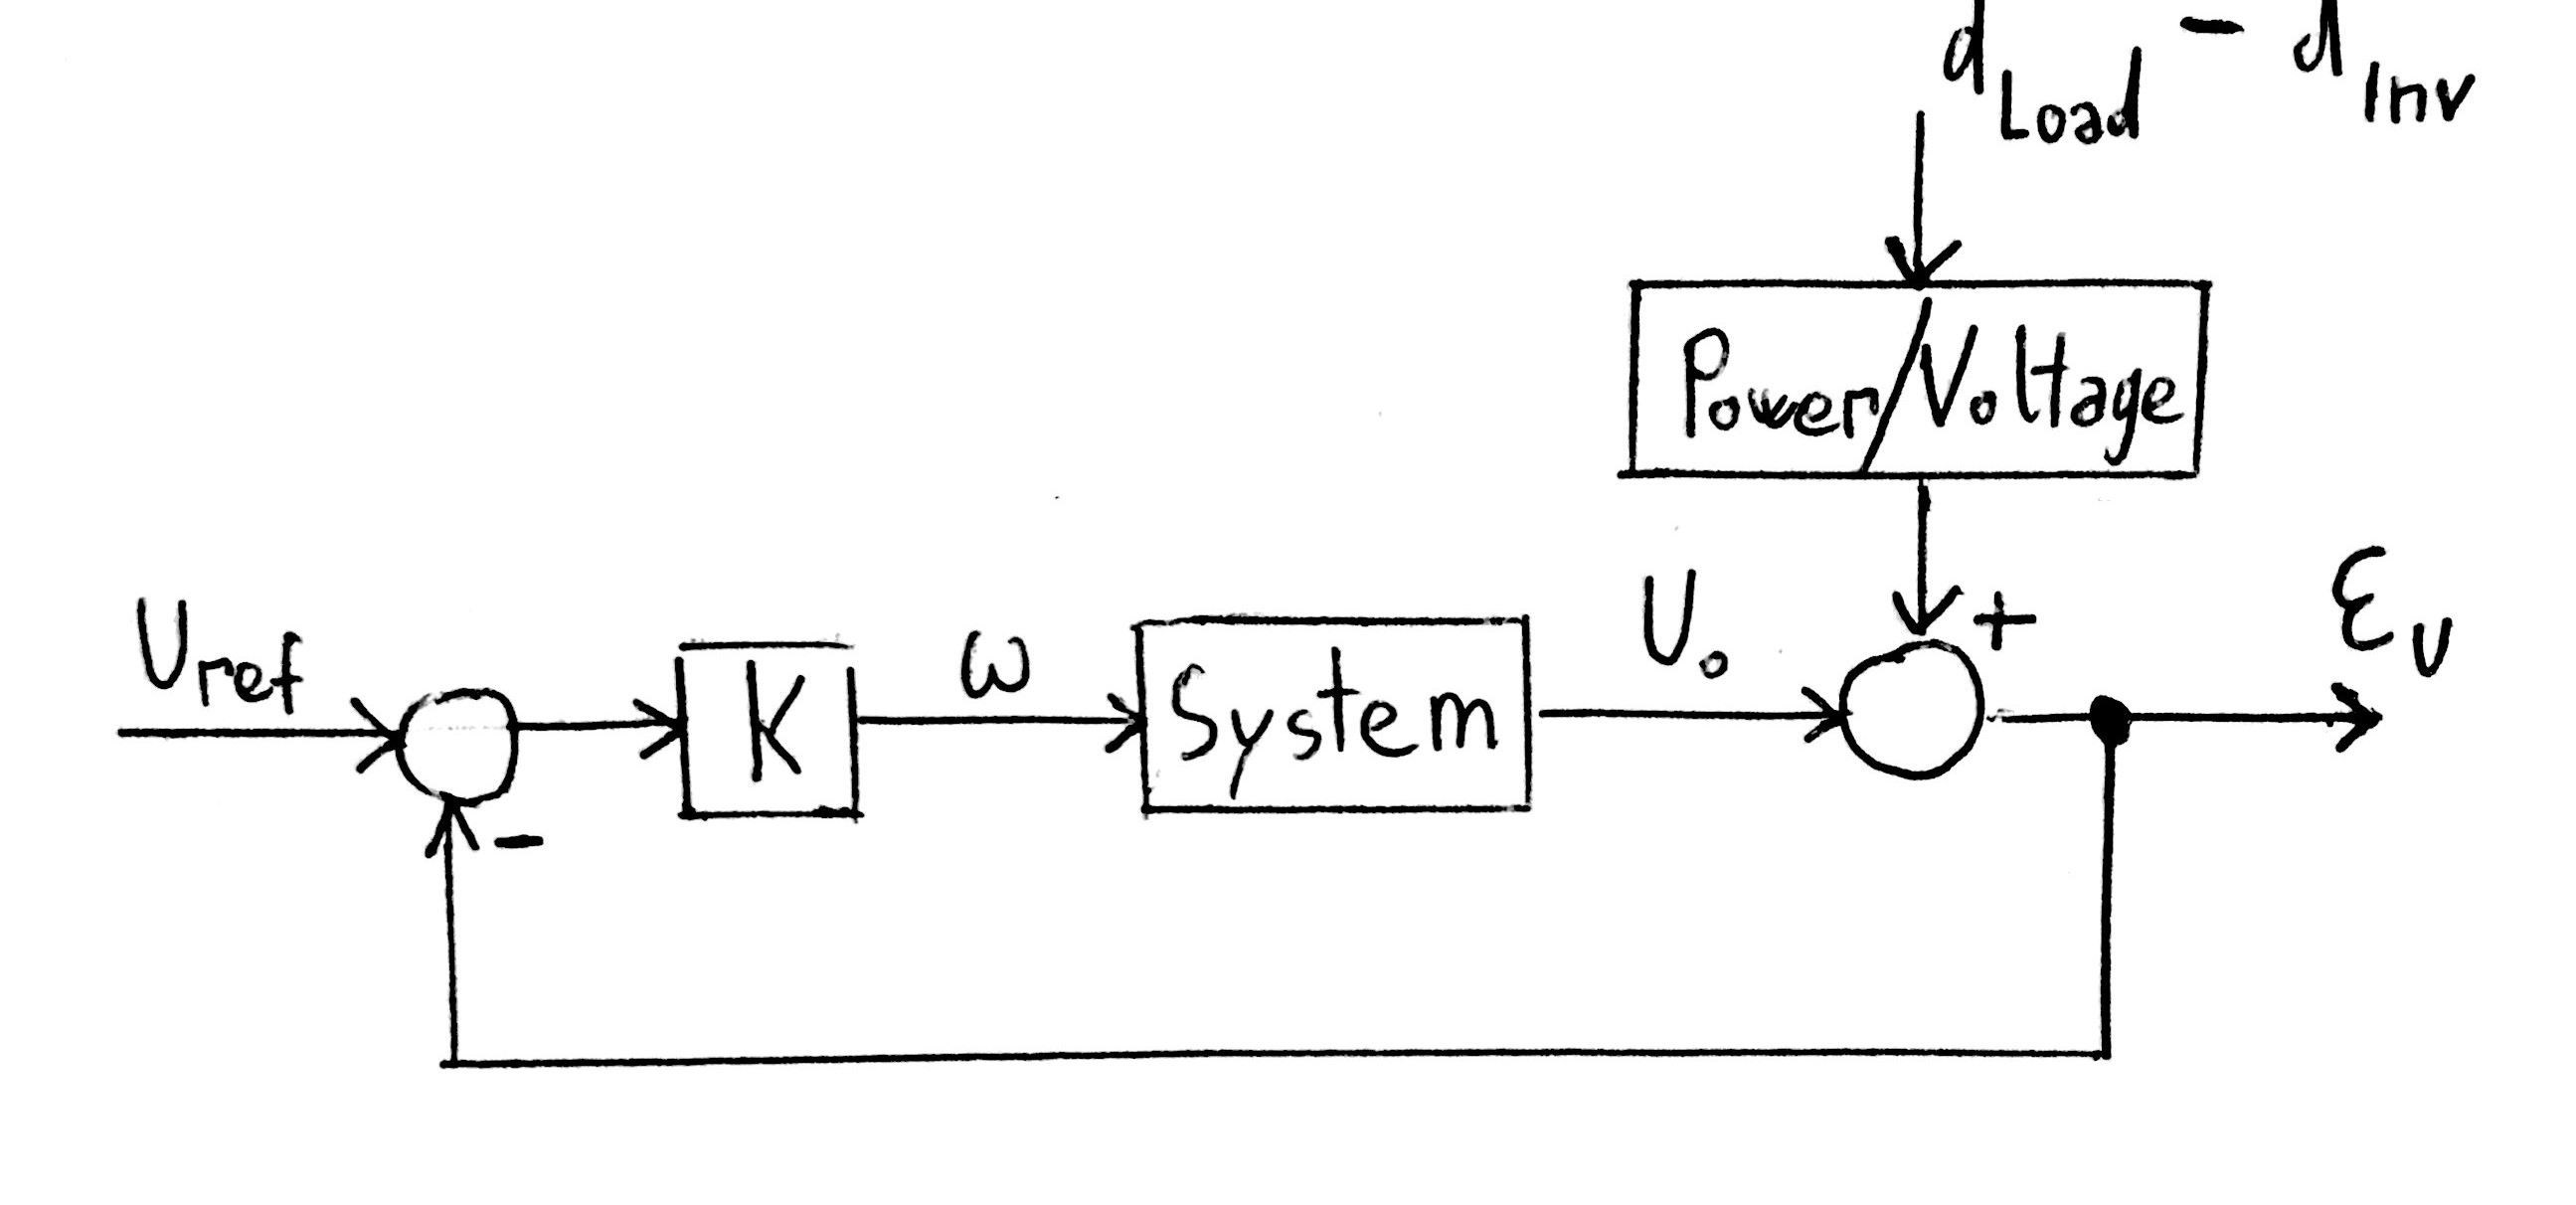
\includegraphics[width=0.65\textwidth]{rapport/billeder/blok_simplified}
%\caption{Simplified closed-loop system for the genset}
%\label{fig:blok_simplified}
%\end{figure}

\begin{figure}[H]
\centering
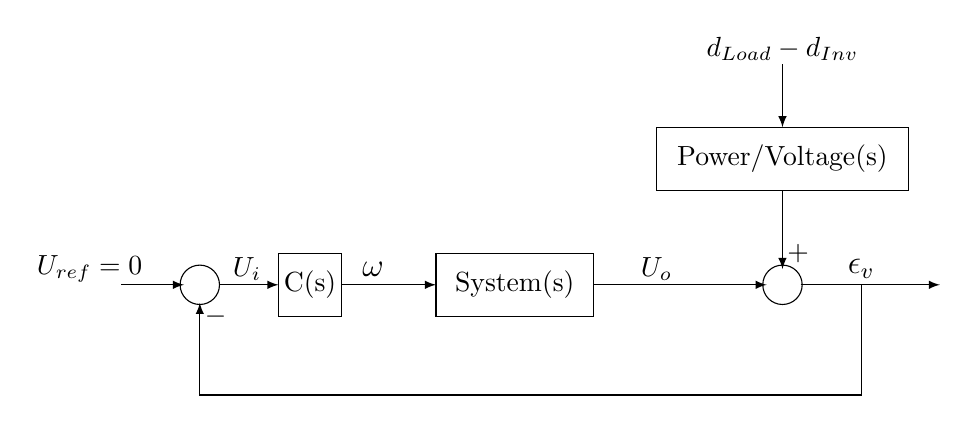
\begin{tikzpicture}

\draw  (-4.8,2.4) rectangle (-2.8,1.6);

\draw [-latex] (-2,4) rectangle (1.2,3.2);

\node at (-0.4,3.6) {\normalsize{Power/Voltage(s)}};
\node at (-3.8,2) {\normalsize{System(s)}};
\node at (-2,2.2) {\normalsize{$U_o$}};
\draw [-latex] (-0.4,2) ellipse (0.25 and 0.25);
\draw [-latex](-2.8,2) -- (-0.6,2);
\draw [-latex](-0.4,3.2) -- (-0.4,2.2);
\draw [-latex] (-6.8,2.4) rectangle (-6,1.6);
\node at (-6.4,2) {C(s)};
\draw [-latex](-6,2) -- (-4.8,2);
\node at (-5.6,2.2) {\large{$\omega$}};
\node at (-0.2,2.4) {$+$};
\draw [-latex] (-7.8,2) ellipse (0.25 and 0.25);
\draw [-latex](-7.54,2) -- (-6.8,2);
\draw [-latex](-0.4,4.8) -- (-0.4,4);
\node at (-0.4,5) {$d_{Load}-d_{Inv}$};
\draw [-latex](-8.8,2) -- (-8,2);
\node at (-9.2,2.2) {\normalsize{$U_{ref} = \footnotesize{0}$}};
\draw [-latex](-0.17,2) -- (1.6,2);
\node at (0.6,2.2) {\large{$\epsilon_v$}};
\draw [-latex](0.6,2) -- (0.6,0.6) -- (-7.8,0.6) -- (-7.8,1.77);
\node at (-7.6,1.6) {$-$};
\node at (-7.2,2.2) {\normalsize{$U_i$}};
\end{tikzpicture}
\caption{Simplified closed-loop system of the genset.}
\label{fig:blok_simplified}
\end{figure}

The subsystem denoted by 'System' is the plant, in other words, the transfer function derived between the mechanical angular velocity and the voltage output of the genset.


\begin{minipage}[t]{0.20\textwidth}
Where\\
\hspace*{8mm} $\omega$ \\
\hspace*{8mm} $U_o$ \\
\hspace*{8mm} $U_i$ \\
\hspace*{8mm} $U_{ref}$ \\
\hspace*{8mm} $d_{Load}-d_{Inv}$ \\
\hspace*{8mm} and $\epsilon_U$ 
\end{minipage}
\begin{minipage}[t]{0.68\textwidth}
\vspace*{2mm}
is the angular velocity output of the controller,\\
is the output voltage of the genset, \\
is the input voltage signal of the controller, \\
is the reference for the system, \\
is the disturbance affecting the system , \\
is the change(error) in the output voltage of the closed-loop controlled system. 

\end{minipage}
\begin{minipage}[t]{0.10\textwidth}
\vspace*{2mm}
\textcolor{White}{te}$\unit{\frac{rad}{s}}$\\
\textcolor{White}{te}$\unit{V}$\\
\textcolor{White}{te}$\unit{V}$\\
\textcolor{White}{te}$\unit{V}$\\
\textcolor{White}{te}$\unit{W}$\\
\textcolor{White}{te}$\unit{V}$
\end{minipage}

The block called 'Power/Voltage' serves as a conversion from power to voltage, since the disturbance applied to the system is in watts. Furthermore, it should be noted that the controller takes an input as voltage and creates a modified angular velocity input for the plant. Therefore the plant can be described as a SISO(Single Input Single Output) system according to the transfer funtion in \eqref{eq:tf_system}. 

\begin{equation}
\label{eq:tf_system}
G_{System}(s) = \frac{U_o(s)}{\omega(s)} = \frac {29.27s}{s^2 + 3.4s + 52.5} \unit{\cdot}
\end{equation}

The simplified plant will now be used to develop the controller. 
  
